%%% License: Creative Commons Attribution Share Alike 4.0 (see https://creativecommons.org/licenses/by-sa/4.0/)
%%% Slides are based heavily on earlier versions of this course taught by Jesper Rudiger.

\documentclass[english,10pt
%,handout
,aspectratio=169
]{beamer}
%%% License: Creative Commons Attribution Share Alike 4.0 (see https://creativecommons.org/licenses/by-sa/4.0/)
%%% Slides are based heavily on earlier versions of this course taught by Jesper Rudiger and Peter Norman Sorensen.

\DeclareGraphicsExtensions{.eps, .pdf,.png,.jpg,.mps,}
\usetheme{reMedian}
\usepackage{parskip}
\makeatother

\renewcommand{\baselinestretch}{1.1} 

\usepackage{amsmath, amssymb, amsfonts, amsthm}
\usepackage{enumerate}
\usepackage{hyperref}
\usepackage{url}
\usepackage{bbm}
\usepackage{color}

\usepackage{tikz}
\usepackage{tikzscale}
\newcommand*\circled[1]{\tikz[baseline=(char.base)]{
		\node[shape=circle,draw, inner sep=-20pt] (char) {#1};}}
\usetikzlibrary{automata,positioning}
\usetikzlibrary{decorations.pathreplacing}
\usepackage{pgfplots}
\usepgfplotslibrary{fillbetween}
\usepackage{graphicx}

\usepackage{setspace}
%\thinmuskip=1mu
%\medmuskip=1mu 
%\thickmuskip=1mu 


\usecolortheme{default}
\usepackage{verbatim}
\usepackage[normalem]{ulem}

\usepackage{apptools}
\AtAppendix{
	\setbeamertemplate{frame numbering}[none]
}
\usepackage{natbib}



\title{Financial Markets Microstructure \\ Lecture 14}

\subtitle{Market Transparency\\
	Chapter 8 of FPR}

\author{Egor Starkov}

\date{K{\o}benhavns Unversitet \\
	Spring 2021}


\begin{document}
\AtBeginSection[]{
\frame<beamer>{
\frametitle{This lecture:}
\tableofcontents[currentsection,currentsubsection]
}}
\frame[plain]{\titlepage}

%\section{Revision and problems}

\begin{frame}{Previously on FMM}
	\begin{itemize}
		\item \structure{Fragmentation} is ubiquitous 
		\item It is costly for uninformed traders, who would prefer to coordinate on a single market
		\item Other costs may include less risk sharing and less competition among traders (see book)
		\item Some benefits are possible (larger depth), depending on setting and trading format
	\end{itemize}
\end{frame}


\begin{frame}{Today: Market transparency}
	\begin{itemize}
		\item Financial markets are among the more transparent ones
		\begin{itemize}
			\item Historical price and transaction data often available
		\end{itemize}
		\item But there are a ways to go
		\begin{itemize}
			\item Often you do not know the price at which your trade will be executed.
		\end{itemize}
		\bigskip\pause
		\item Today: discuss how transparency affects market outcomes
		\item Related to last week's discussions
		\item Different kinds of transparency have different effects
	\end{itemize}
\end{frame}


\begin{frame}{Market transparency: introduction}
	\begin{columns}
		\begin{column}{0.6\linewidth}
			{\setstretch{1.3}
			\begin{itemize}
				\item Market transparency can refer to different information
				\begin{itemize}
					\item \textbf{Pre-trade information}: quotes and limit orders
					\item \textbf{In-trade information}: trader identity
					\item \textbf{Post-trade information}: realized trades and prices
				\end{itemize}
				\pause
				\item Exchanges profit from selling this type of data
				\begin{itemize}
					\item Different traders end up with different information sets
					\item Some types of traders may benefit from a lack of transparency
				\end{itemize}
			\end{itemize}
			}
		\end{column}
		\begin{column}{0.4\linewidth}
			\pause[1]
			\includegraphics<handout:0>[width=\linewidth]{pics/transparency}
		\end{column}
	\end{columns}
\end{frame}


\begin{frame}{Market transparency: regulation}
	\begin{columns}
		\begin{column}{0.6\linewidth}
			{\setstretch{1.3}
			Transparency also \structure{regulated}
				\begin{itemize}
					\item In both Europe and the US: rules to assure pre-trade information
					\item Also, firms must disclose relevant information
					\item The US has a centralized system for collecting post-trade information, but not Europe
				\end{itemize}
			}
		\end{column}
		\begin{column}{0.4\linewidth}
			\pause[1]
			\includegraphics<handout:0>[width=\linewidth]{pics/transreg}
		\end{column}
	\end{columns}
\end{frame}


\begin{frame}[label=ideas]
	\frametitle{General ideas}
	\begin{enumerate}
		\item In an opaque market, search costs confer monopoly powers to dealers
		\item Transparency may foster competition, but also collusion
		\item Risk-sharing may be better when markets are opaque
	\end{enumerate}
	\hyperlink{example}{\beamerbutton{An (extreme) example of poorly informed trading}}
\end{frame}



\section{Pre-trade transparency}

\begin{frame}{Quote transparency}
	\begin{itemize}
		\item In some markets LOB and dealer quotes are visible (possibly at a cost)
		\item In some other (esp. illiquid) markets trader must search for quotes 
		\begin{itemize}
			\item or approach dealers in search of price improvements
		\end{itemize}
		\item (This was the problem 3 in PS1)
	\end{itemize}
\end{frame}


\begin{frame}{Search costs}
	Idea based on Diamond's (1971) \structure{chain store paradox}
	\begin{itemize}
		\item Imagine a product market with consumers and firms
		\item Firms set prices not initially seen to consumers
		\item Suppose consumers are searching stores sequentially to find the best price, searching costs $c$ per store
		\item Look for an equilibrium in which all stores set same price $p$
		\item Each store has market power: can charge customer up to $p+c$ if desired
		\item \textbf{Equilibrium}: stores set $p$ at monopoly level
	\end{itemize}
\end{frame}


\begin{frame}{Search costs}
	\begin{itemize}
		\item The situation is the same in a financial market with search cost
		\begin{itemize}
			\item It doesn't pay to be the cheapest dealer -- can't advertise price
			\item Can always increase price and still be preferred due to search cost
		\end{itemize}
		\item Model conclusion does not depend on size of search cost (ignore what textbook says about it)
		\begin{itemize}
			\item Although irl frictions probably increase in search cost -- fancier models capture this
		\end{itemize}
		\item \structure{Welfare} implications:
		\begin{itemize}
			\item \alert{Dealers} have market power $\Rightarrow$ \alert{higher profits}
			\item All \alert{traders are worse off}, the less sophisticated ones more so
		\end{itemize}
	\end{itemize}
\end{frame}


\begin{frame}{Quote transparency}
	\begin{itemize}
		\item Let's look at another dimenstion of quote transparency
		\item While price of the first unit is often observable...
		\begin{itemize}
			\item US protects NBBO orders for each stock
			\item Exchanges or dealers may only quote best bid\&ask
		\end{itemize}
		\item But \structure{depth} is more difficult to gauge
		\item If depth is volatile (which it is), may trade at the ``wrong time''
	\end{itemize}
\end{frame}


\begin{frame} [label=quotes]
	\frametitle{Uncertainty and price sensitivity}
	\begin{itemize}
		\item Consider a Kyle model with random depth $\lambda$.
		\item \textbf{Transparent market}: insider demand is inversely related to price sensitivity $\lambda$: $x^T \sim \frac{1}{\lambda}$
		\item \textbf{Opaque market}: traders face uncertainty, so their demand is inversely related to expected price sensitivity: $x^O \sim \frac{1}{\mathbb{E}(\lambda)}$
		\item Convex function. Use Jensen's inequality: 
		\[
		\mathbb{E}\left(\frac{1}{\lambda}\right) > \frac{1}{\mathbb{E}(\lambda)}
		\]
		\item \structure{More trading in transparent market}
		\begin{itemize}
			\item Risk of high $\lambda$ provides stronger incentive to reduce $x$ than the incentive to increase $x$ from the chance of low $\lambda$.
		\end{itemize}
	\end{itemize}
\end{frame}


\begin{frame}{Order flow transparency}
	\begin{columns}
		\begin{column}{0.6\linewidth}
			{\setstretch{1.3}
				\begin{itemize}
					\item In some markets (OTC, FX) an order may be filled simultaneously by different liquidity providers
					\item What does it matter if they can or cannot observe the whole order flow?
					\pause
					\begin{itemize}
						\item We saw one answer already (Glosten vs Kyle)
						\item Will now look at another way to model this
					\end{itemize}
				\end{itemize}
			}
		\end{column}
		\begin{column}{0.4\linewidth}
			\pause[1]
			\includegraphics<handout:0>[width=0.8\linewidth]{pics/cheating}
		\end{column}
	\end{columns}
\end{frame}


\begin{frame}{Order flow: Model}
	\begin{itemize}
		\item \textbf{Value}: high $v^H$ or low $v^L$ with equal probability
		\begin{itemize}
			\item Mean: $\mu=(v^H+v^L)/2$
		\end{itemize}
		\item \textbf{Dealers}: set quotes, competitive, risk neutral
		\item \textbf{Traders}: two traders arrive, submit unit market orders
		\begin{itemize}
			\item With prob. $\pi$: both are informed
			\item With prob. $1-\pi$: both liquidity traders;  one seller, one buyer
		\end{itemize}
		\item \textbf{Crucial assumption}: previous point implies higher order flow correlation  when traders are informed. Intuition: 
		\begin{itemize}
			\item Informed traders: suppose all learn that the asset value is, say, high, we should all want to buy
			\item Liquidity traders: suppose pension fund decides it wants a less risky portfolio. (Probably) uncorrelated with other liquidity traders' decisions
		\end{itemize}
	\end{itemize}
\end{frame}


\begin{frame}{Order flow: Equilibrium}
	\begin{itemize}
		\item \textbf{Opaque}: dealers quote without seeing the entire market order flow
		\begin{itemize}
			\item As in chapter 3, $a^{O}=\mu+\pi(v^{H}-\mu)$ and $b^{O}=\mu-\pi(\mu-v^{L})$
		\end{itemize}
		\item \textbf{Transparent}: dealers condition quotes on both orders
		\begin{itemize}
			\item Two buyers: must be informed, $a^{T}=v^{H}$
			\item Two sellers: must be informed, $b^{T}=v^{L}$
			\item One of each: trade at $\mu$
		\end{itemize}
		\item Transparent ($T$) versus opaque ($O$) market:
		\begin{itemize}
			\item $T$ better than $O$ for uninformed: avoid adverse selection premium
			\item Better price discovery in $T$ than in $O$:  private information revealed
			\item Note: informed order flow may be endogenously reduced in $T$, and then above analysis loses power
		\end{itemize}
	\end{itemize}
\end{frame}



\section{Post-trade transparency}

\begin{frame}{Post-trade transparency}
	\begin{itemize}
		\item If orders arrive sequentially, what effect does information about past orders have?
		\item \textbf{Value}: high $v^H$ or low $v^L$ with equal probability
		\begin{itemize}
			\item Mean: $\mu=(v^H+v^L)/2$
		\end{itemize}
		\item \textbf{Dealers}: set quotes, competitive, risk neutral
		\item \textbf{Traders}: two traders arrive, submit unit market orders
		\begin{itemize}
			\item With prob. $\pi$: both are informed
			\item With prob. $(1-\pi)/2$: both liquidity traders;  first  seller, then buyer
			\item With prob. $(1-\pi)/2$: both liquidity traders;  first  buyer, then seller
		\end{itemize}
		\item \textbf{Transparent market}: All dealers observe the first order $y_1$
		\begin{itemize}
			\item Set $a_1=\mu+\pi(v^{H}-\mu)$ and $a_{2y_1}=\mathbb{E}[v|y_1,buy]$
		\end{itemize}
	\end{itemize}
\end{frame}


\begin{frame}{Post-trade transparency: Period 2}
	\textbf{Opaque market}: First dealer gains informational advantage. Focus on \alert{ask side}
	\begin{itemize}
		\item \structure{Period 2}. Denote the dealer who observed period-1 trade by \alert{$I$}, and the other dealer by \alert{$U$}.
		\begin{itemize}
			\item For technical reasons, suppose $I$ sets price after observing $U$'s quote
			\item \structure{Dealer $U$}: How to quote if you didn't see the first trade and second trade is buy? 
			\begin{itemize}
				\item If you set ask $a^U_2<v^{H}$ you will be undercut by $I$  if first order was a sell
				\item You only get to trade if first order was buy: lose $v^{H}-a^U_2$
				\item Thus, uninformed dealers need to quote $a^U_2=v^{H}$
			\end{itemize}
			\item \structure{Dealer $I$}: Suppose you saw the first trade, and second trade is a buy:
			\begin{itemize}
				\item Set price at $a^I_{2s}=v^{H}$ if first trade was a sell, and $a^I_{2b} = v^H - \epsilon$ if buy
				\item  $I$ wins period-2 buy order if $y_1$ was a sell (otherwise can undercut $U$)
				\item  $U$ wins period-2 buy order if $y_1$ was a buy, since $I$ knows that asset value is high
			\end{itemize}
		\end{itemize}
	\end{itemize}
\end{frame}


\begin{frame}{Post-trade transparency: Period 1}
	\begin{itemize}
		\item \structure{Period 1.} The sequential information advantage uncovered in the previous slide can make dealers bid keenly for the first order
		(Forex dealers often said to quote negative spread to large traders)
		\begin{itemize}
			\item In second period, $I$'s profit is $(1-\pi)(v^{H}-v^{L})/2$. $U$'s profit is zero
			\item Competition leads the first period half-spread to be reduced by this amount, to $(2\pi-1)(v^{H}-v^{L})/2$ (dealers undercut each other to obtain information contained in first order)
			\item The uninformed's aggregate trading cost is $\pi(v^{H}-v^{L})$ - double the cost under transparency. Why is this?
		\end{itemize}
		\item Would dealers commit to transparency?
		\begin{itemize}
			\item No, there is always an incentive to hide your orders (section 8.4.2)
			\item May explain the rise of less transparent trading venues
		\end{itemize}
	\end{itemize}
\end{frame}


\begin{frame}{Post-trade transparency: Collusion}
	\begin{columns}
		\begin{column}{0.6\linewidth}
			{\setstretch{1.3}
				\begin{itemize}
					\item If dealers are not perfectly competitive, they can try to \structure{collude} to increase their profits
					\item Cartels are sustained via a threat of \alert{punishment} in case anyone \alert{deviates}
					\begin{itemize}
						\item Example: Russia went against OPEC last year, so OPEC flooded the market
					\end{itemize}
					\pause
					\item Prerequisite for collusion: ability to detect deviations
					\begin{itemize}
						\item Transparency improves this ability
						\item So may help collusion
					\end{itemize}
				\end{itemize}
			}
		\end{column}
		\begin{column}{0.4\linewidth}
			\pause[1]
			\includegraphics<handout:0>[width=\linewidth]{pics/collusion}
		\end{column}
	\end{columns}
\end{frame}



\section{In-trade information}

\begin{frame}{In-trade information}
	\begin{columns}
		\begin{column}{0.7\linewidth}
			{\setstretch{1.3}
				\begin{itemize}
					\item Transparency may relate not only to quote and order data, but also to \structure{trader identity}.
					\begin{itemize}
						\item LOB is very anonymous and thus opaque
						\item dealer interactions can be personal
					\end{itemize}
					\pause
					\item If trader's identity is visible, it may affect the prices he gets
					\begin{itemize}
						\item Institutional investors rarely engage in informed trading, so will get good price;
						\item Insiders will get bad prices.
						\item See the figure for FX market on the next slide (from \cite{ranaldo_asymmetric_2019})
					\end{itemize}
					\pause
					\item If identity is limited to some identifier in the system, trader can still build a reputation through history of actions
				\end{itemize}
			}
		\end{column}
		\begin{column}{0.3\linewidth}
			\pause[1]
			\includegraphics<handout:0>[width=\linewidth]{pics/incognito}
		\end{column}
	\end{columns}
\end{frame}


\begin{frame}
	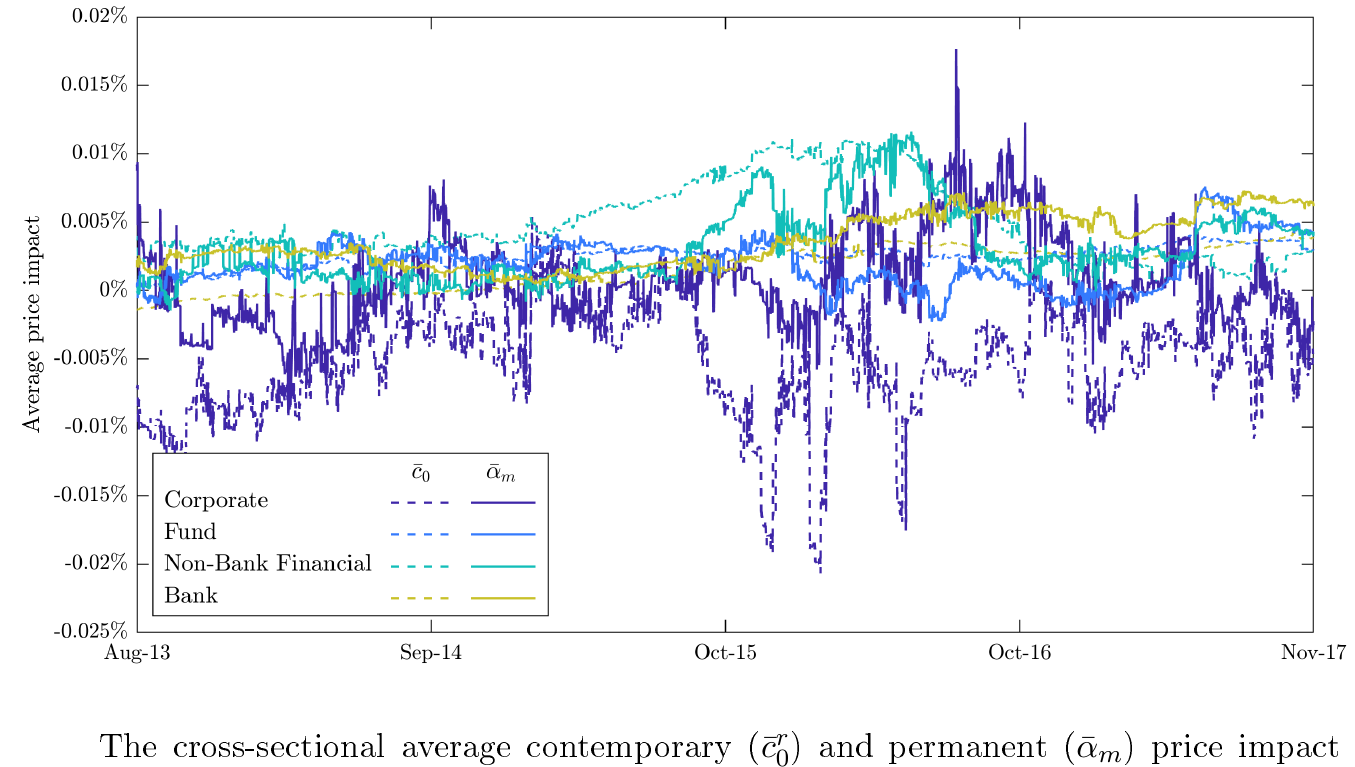
\includegraphics[width=\linewidth]{pics/RS}
\end{frame}


\begin{frame}{In-trade information}
	\begin{itemize}
		\item There may be ways to signal or credibly \structure{disclose} the fact that your \structure{trade is uninformative}
		\begin{itemize}
			\item E.g. can advertise trade a few days in advance -- ``sunshine trading''
		\end{itemize}
		\item In this case they \emph{will} be used because uninformed traders will want to separate -- \structure{transparency will prevail}
		\item Same may happen due to \alert{cream-skimming}
		\begin{itemize}
			\item Large banks can execute trades in their own dark pools instead of forwarding to the market
			\item They would pick off profitable trades and forward the rest
			\item The market would account for this and react appropriately
		\end{itemize}
	\end{itemize}
\end{frame}


\begin{frame}{In-trade information}
	\begin{itemize}
		\item In all of the above, transparency leads to reallocation of welfare from insiders to the uninformed.
		\begin{itemize}
			\item That's why regulators push for transparency and the market resists
			\item You can also argue that due to this transparency would reduced informed trading and reduce price discovery
		\end{itemize}
		\item Hirshleifer noted that some risk-sharing trades are better conducted before information arrives
		\begin{itemize}
			\item Think of health insurance
			\item Possible to share risks before we know who suffers illness
			\item Too late to share risks after the illness is known; market break-down
		\end{itemize}
	\end{itemize}
\end{frame}


\begin{frame}{Conclusion}
	\begin{itemize}
		\item \structure{Transparency} mostly reallocates welfare across market participants 
		\begin{itemize}
			\item Uninformed traders benefit, so T \structure{helps liquidity}
			\item Insiders may lose, so T \structure{worsens price discovery}
			\item Dealers may win or lose
		\end{itemize}
		\item But transparency may also impede risk sharing, and have adverse effects when it is asymmetrically distributed
		\item Opaqueness can be good in limit books
		\begin{itemize}
			\item Hidden limit orders help uninformed traders hedge their positions where making these orders visible would by itself create adverse price movements
		\end{itemize}
	\end{itemize}
\end{frame}


\begin{frame}{Exercise for next week}
	\begin{itemize}
		\item Read the article on Mifid-2 (on Absalon). Discuss the following questions:
		\begin{itemize}
			\item What did Mifid2 change in regards to market transparency? (There are many aspects to this.) How will these changes affect market outcomes?
		\end{itemize}
		\item Read the article on LSE acquiring Refinitiv. What implications can this have for market transparency (e.g. on LSE's own trading platform)?
		\item Do ex.2 after ch.8 (p.303) on price discovery
	\end{itemize}
\end{frame}


\appendix
\begin{frame}<handout:0>[allowframebreaks]{References}
	\bibliography{../teaching}
	\bibliographystyle{abbrvnat}
\end{frame}


\begin{frame}[label=example]{Aspiro}
	\begin{itemize}
		\item Some years ago, Jay-Z bought Swedish music service Aspiro   
		\pause
		\begin{center}
			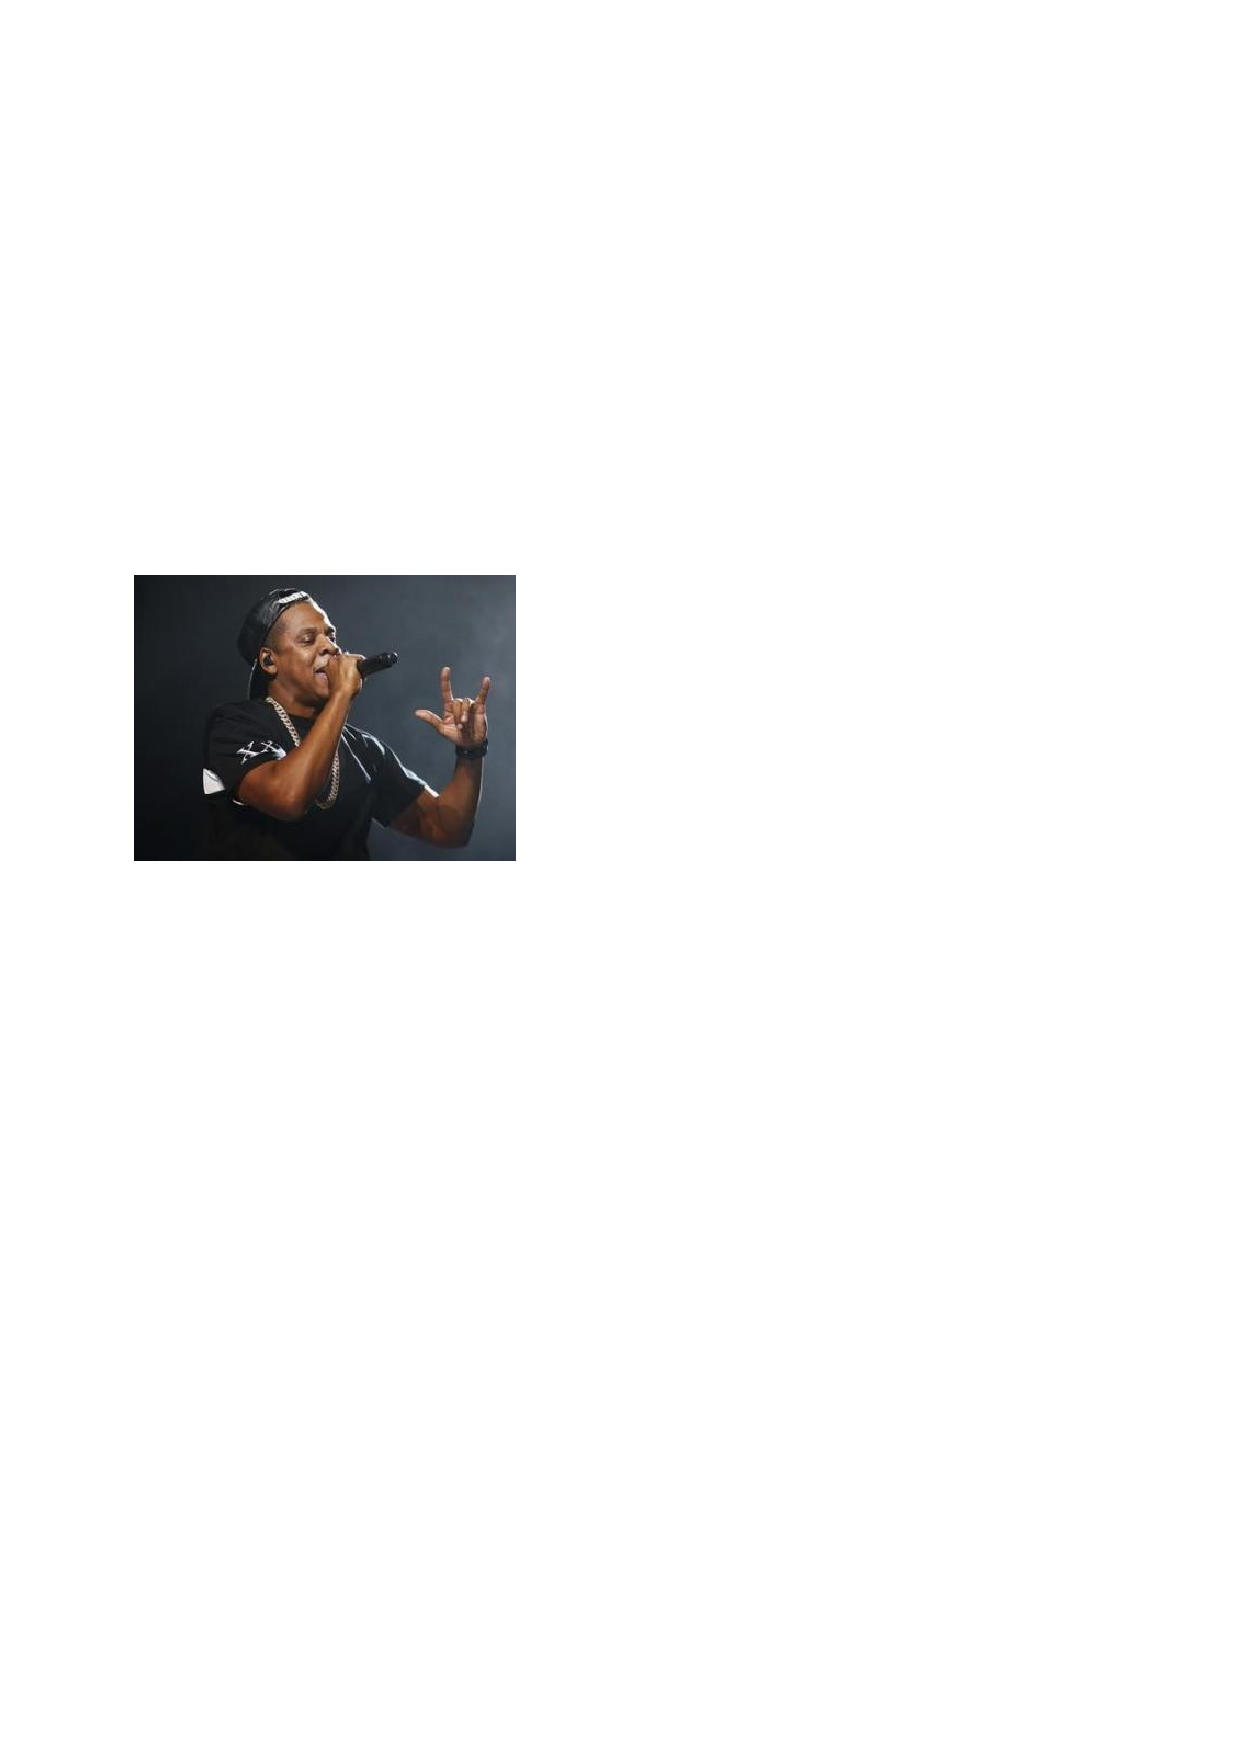
\includegraphics[width=.25\paperwidth]{pics/jayz}
		\end{center}
	\end{itemize}
\end{frame}


\begin{frame}<handout:0>{Aspiro}
	\begin{itemize}
		\item Shortly after they launched their new service `Tidal'
		\pause
		\begin{center}
			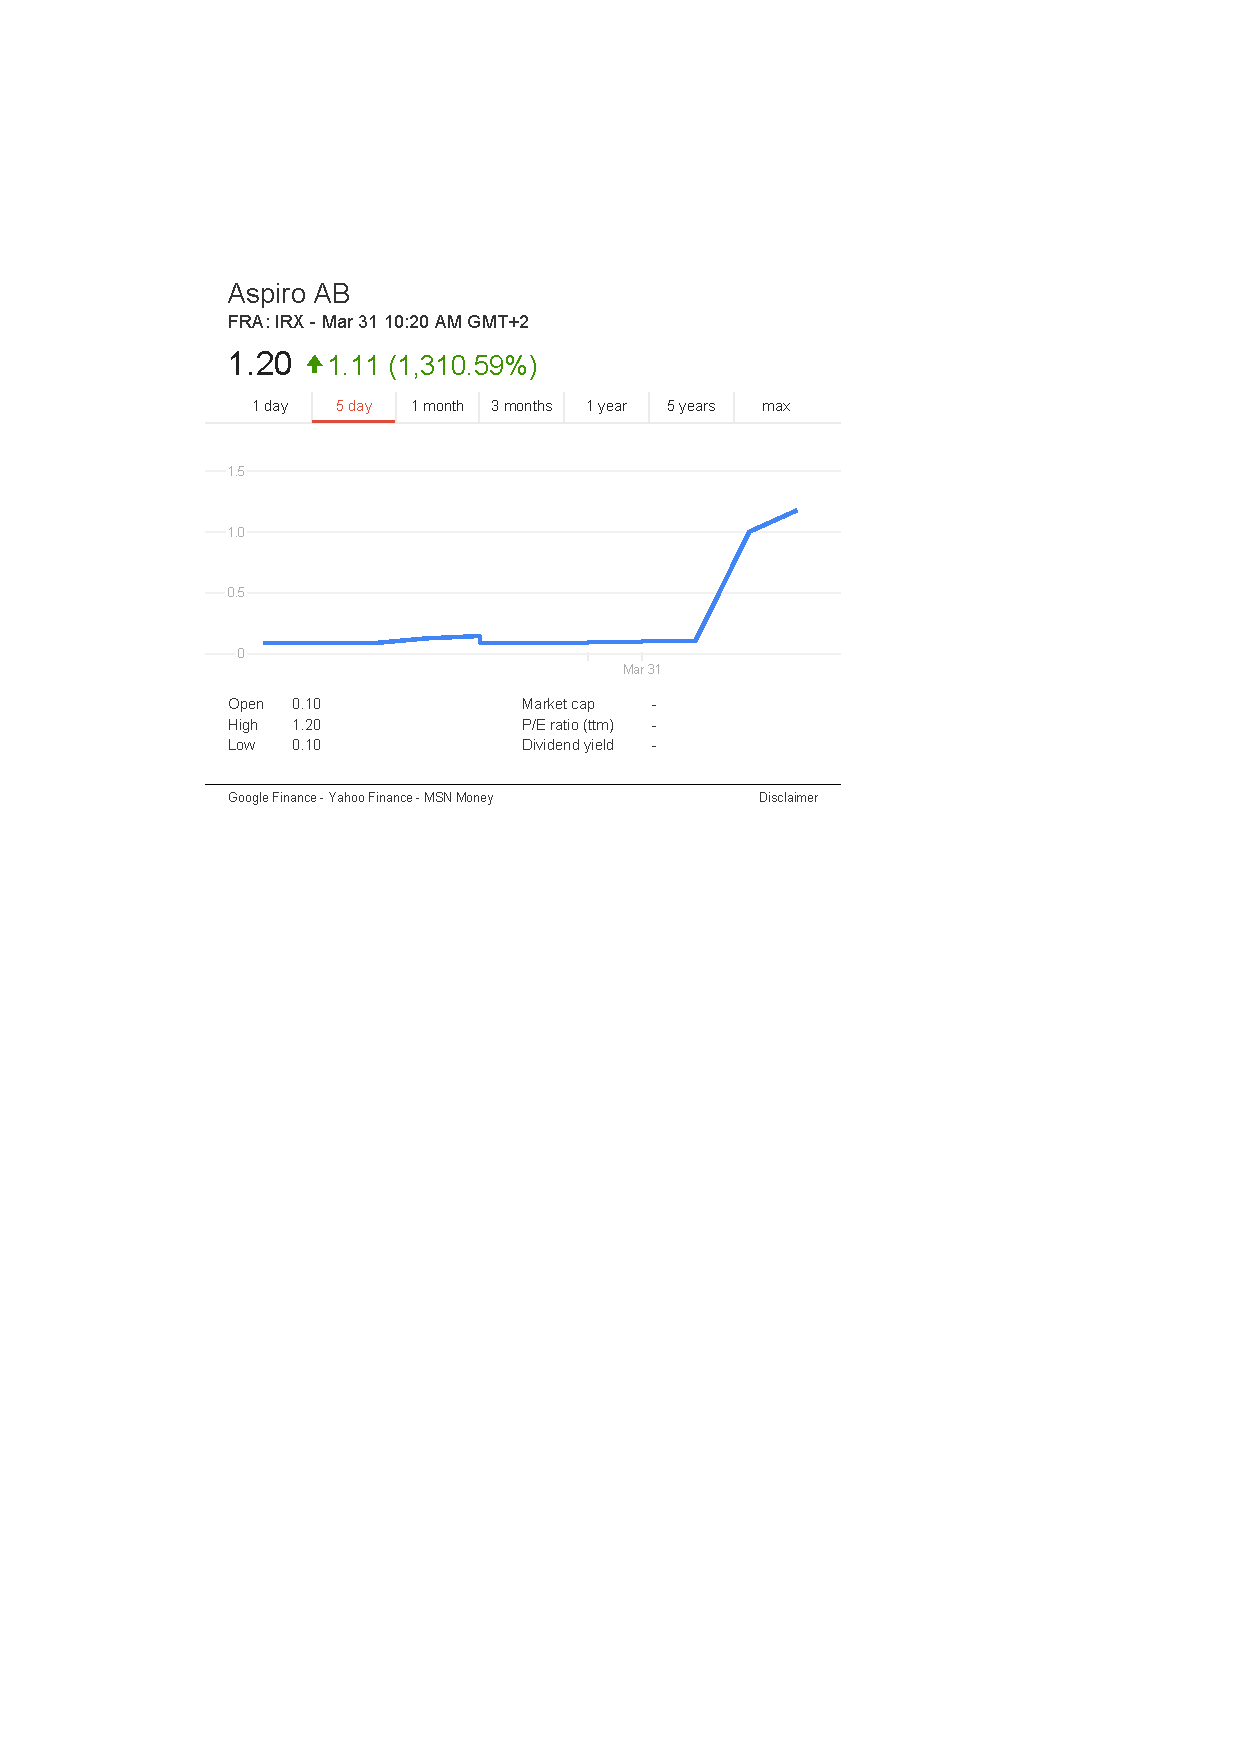
\includegraphics[width=0.5\paperwidth]{pics/aspiro}
		\end{center}
	\end{itemize}
\end{frame}


\begin{frame}<handout:0>{Aspiro}
	\begin{itemize}
		\item There was one caveat though...
		\begin{itemize}
			\item Since Jay-Z bought more than 90\% of the stock, the remaining owners must sell to him at same price as he bought the first stock (so that he can delist the firm)
			\item Meaning that they must all sell to him at price SEK 1.05
			\pause
			\item The day before this forced trade was due to be executed, trading was halted by the exchange when the price was at SEK 11.00
			\item Traders seemed unaware of this rule or unaware that Jay-Z had acquired enough stock to trigger the rule, so OMX Stockholm issued to two notices and phoned brokers
			\item Let's see what happened
		\end{itemize}
	\end{itemize}
\end{frame}


\begin{frame}<handout:0>{Aspiro}
	First trading halt
	
	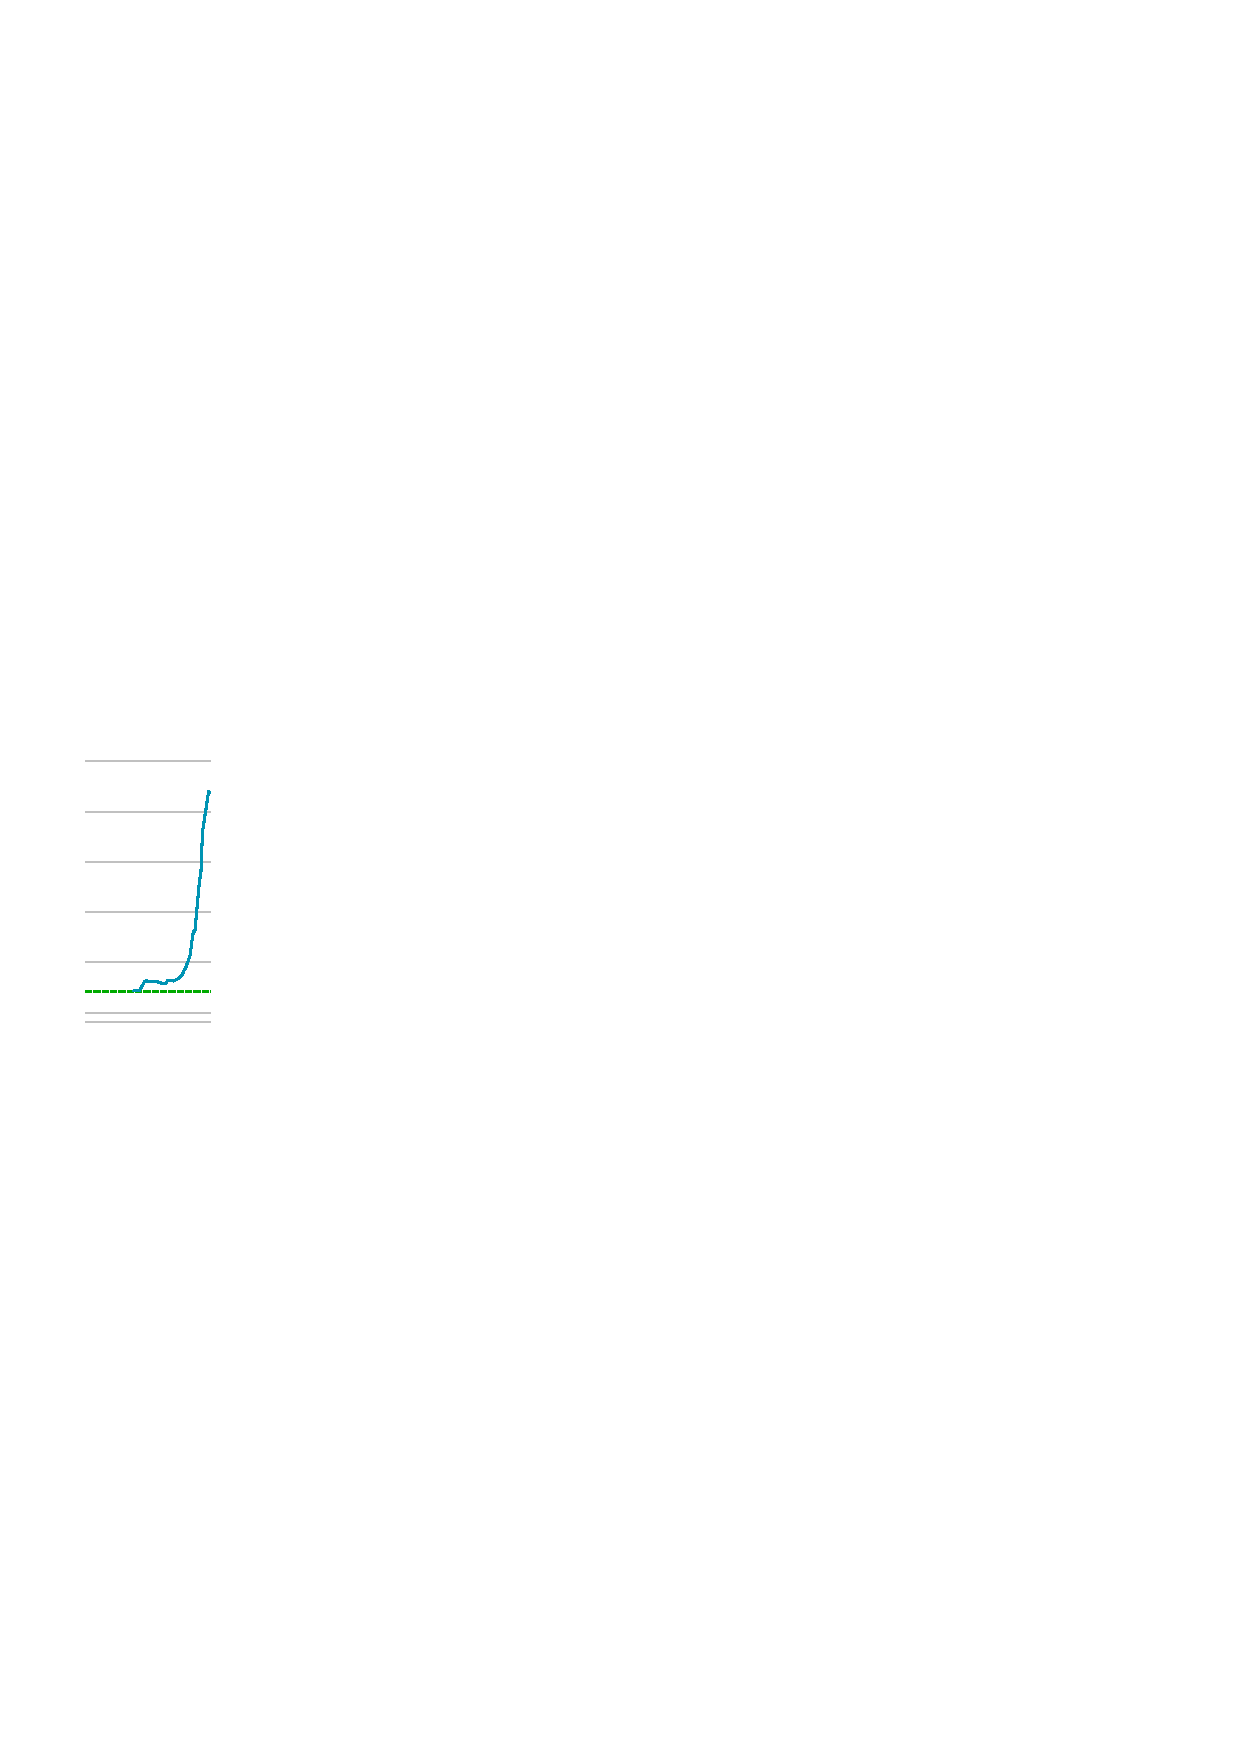
\includegraphics{pics/aspiro1}
\end{frame}


\begin{frame}<handout:0>{Aspiro}
	Brokers are phoned and price is adjusted
	
	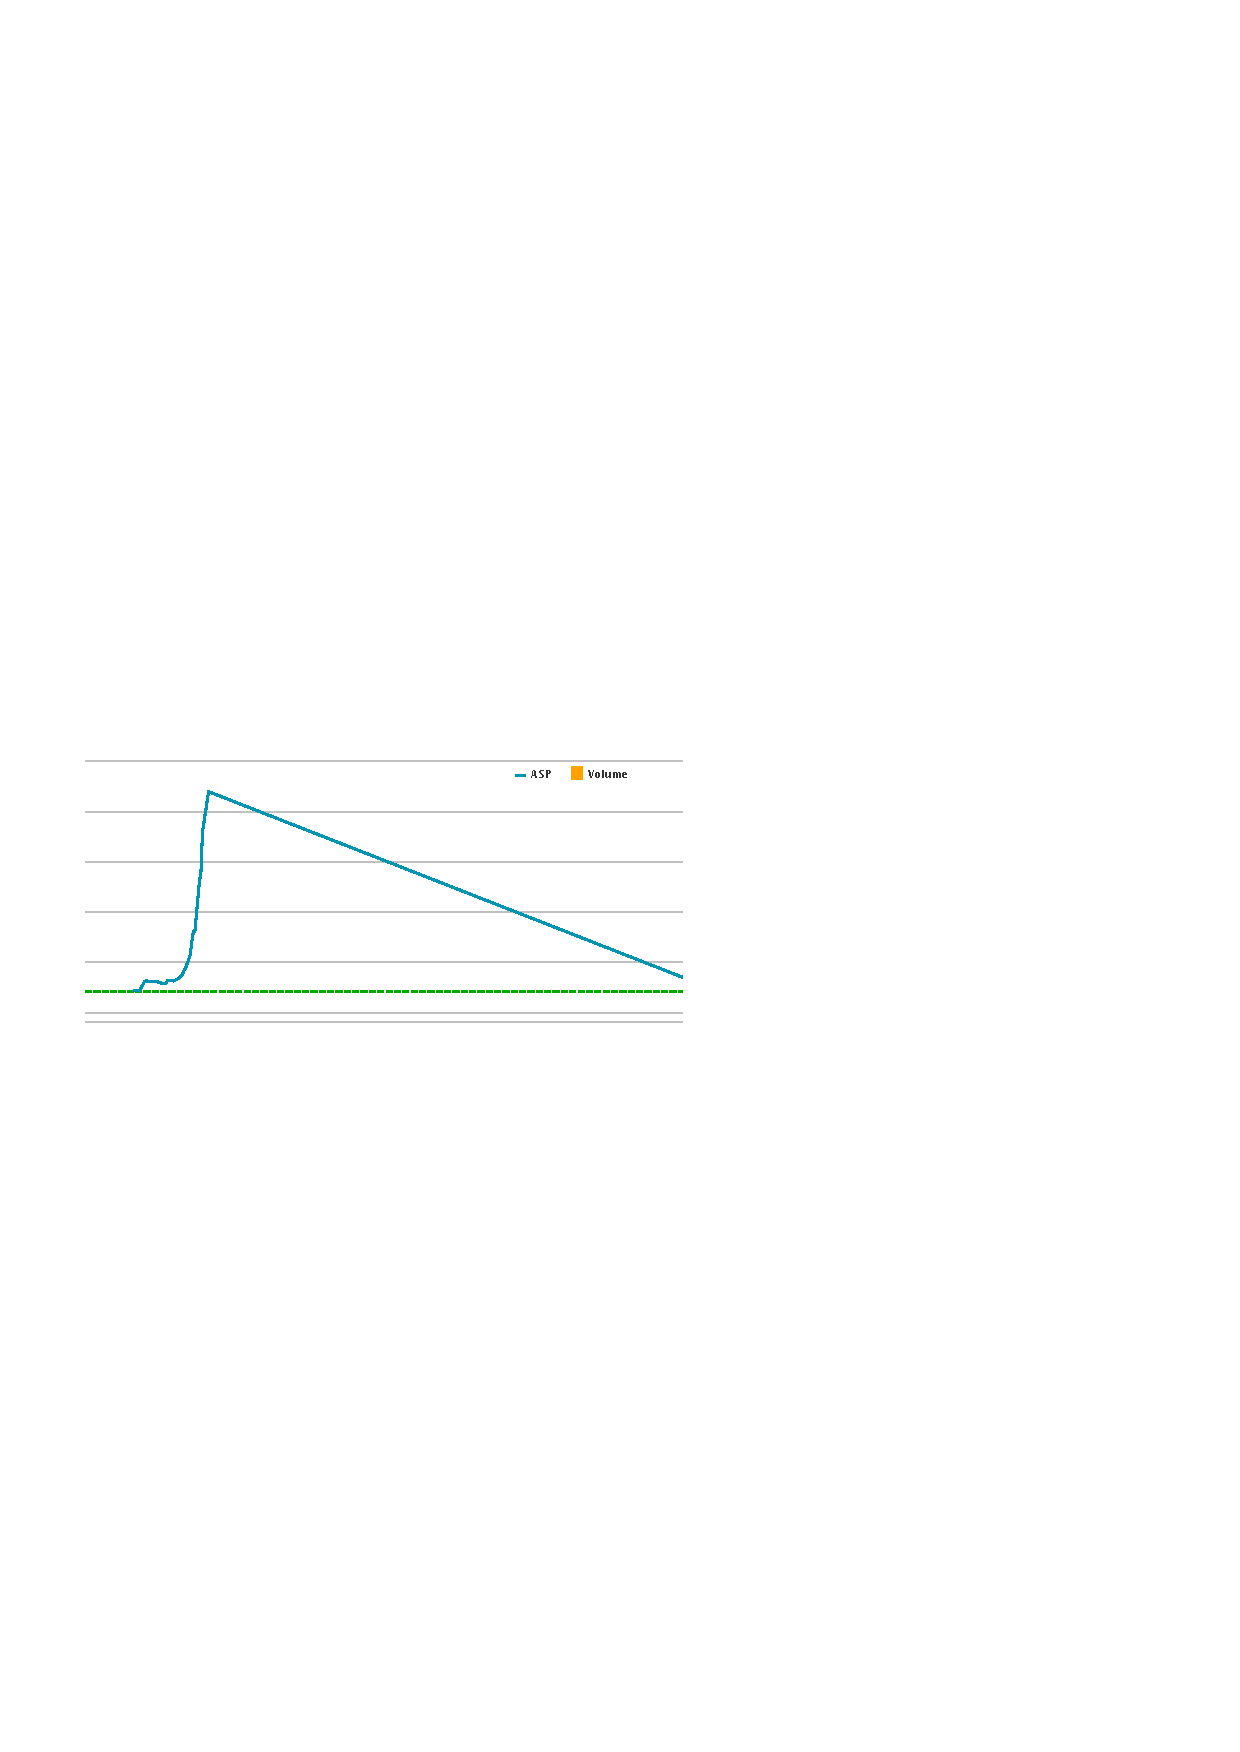
\includegraphics{pics/aspiro2}
\end{frame}


\begin{frame}<handout:0>{Aspiro}
	Trading resumes...
	
	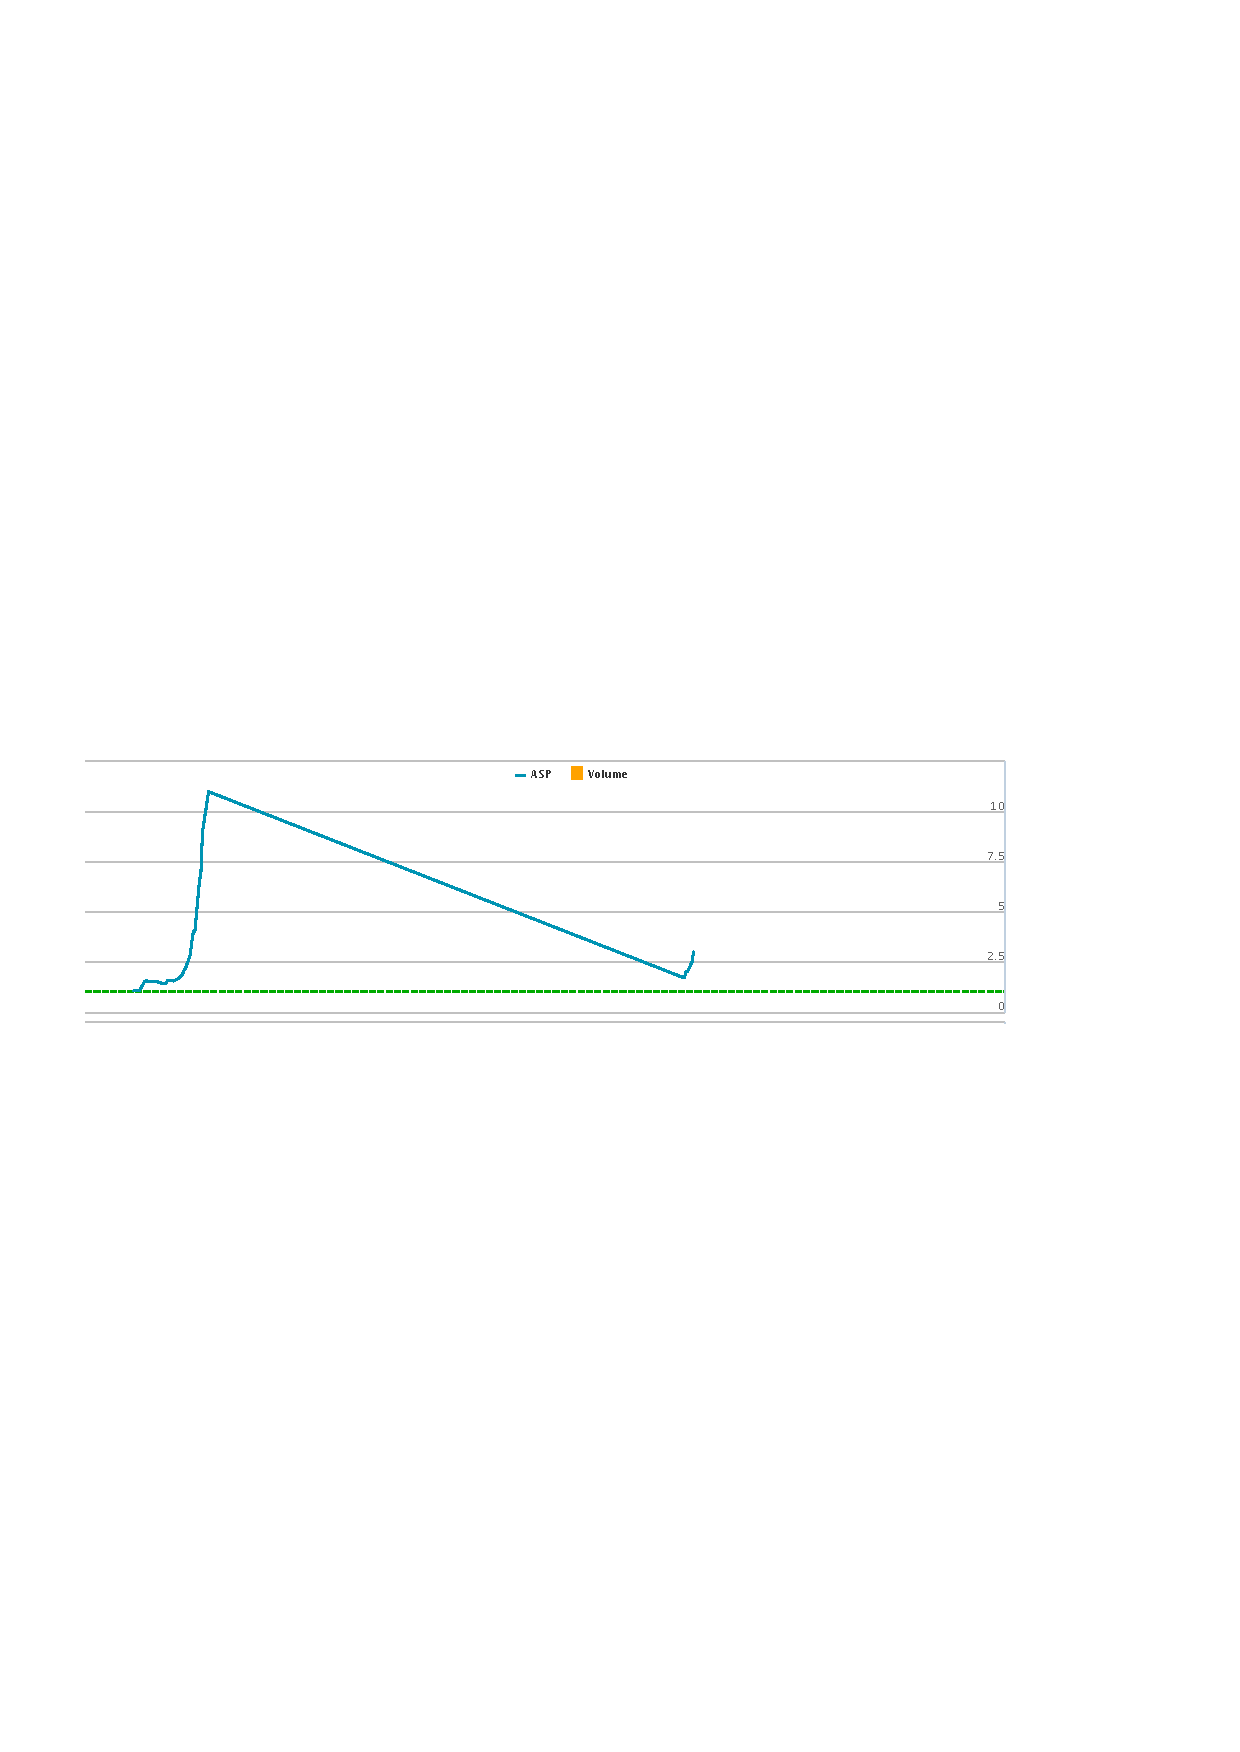
\includegraphics[width=0.85 \paperwidth]{pics/aspiro3}
	\pause
	The stock immediately started trading at 3 times tomorrow's forced bid price, and was closed down again.
	\pause 
	Sometimes, even the most basic and readily available information can be opaque to some traders.
	\hyperlink{ideas}{\beamerbutton{Back}}
\end{frame}


%\begin{frame}[label=convexity]
%	\frametitle{Why the convexity?}
%	\begin{itemize}
%		\item Price schedule is given by $p(x) = \mu+\lambda x$ 
%		and value  by $v=\mu+\varepsilon$
%		\item Trader solves $\max_x \{ \mathbb{E} [ (\varepsilon-\lambda q) x] \}$ to get $x^*=\frac{\varepsilon}{2\lambda}$
%		\item To understand, take derivative of profit impact with respect to $\lambda$
%		\[
%		\frac{ \partial^2 (\varepsilon x - \lambda x^2)}{\partial x \partial \lambda} = -2x
%		\]
%		\item $\lambda \downarrow$ : lower price on many units
%		\item $ \lambda \uparrow$ : higher price on few(er)  units
%		\item Decreasing $\lambda$ has greater quantity impact than increasing $\lambda$ \hyperlink{quotes}{\beamerbutton{Back}}
%	\end{itemize}
%\end{frame}


\end{document} 